\documentclass[11pt,a4paper]{article}

\usepackage[margin=2.3cm]{geometry}
\usepackage[T1]{fontenc}
\usepackage{lmodern}
\usepackage{graphicx}
\usepackage{booktabs}
\usepackage{tabularx}
\usepackage{float}
\usepackage{caption}
\usepackage{xcolor}
\usepackage{amssymb}
\usepackage{enumitem}
\usepackage[hidelinks]{hyperref}

\definecolor{hanoi}{HTML}{0284C7}
\definecolor{danang}{HTML}{D97706}
\definecolor{hcm}{HTML}{D93856}
\newcommand{\HN}{\textcolor{hanoi}{\textbf{Hanoi}}}
\newcommand{\DN}{\textcolor{danang}{\textbf{Da Nang}}}
\newcommand{\HCM}{\textcolor{hcm}{\textbf{HCMC}}}

\setlist{itemsep=2pt, topsep=4pt}
\emergencystretch=3em
\captionsetup{font=small, labelfont=bf}
\graphicspath{{figures/}}

\title{Temperature Dynamics \& Variations\\[4pt]
\large Research Question 1 -- Exploratory Data Analysis and Visualization Design}
\author{Eva Wimmer (IT26EX013)\\
\small Cross-Regional Weather Dynamics in Vietnam -- Data Science and Data Visualization}
\date{November 2026}

\begin{document}
\maketitle

\begin{abstract}
\noindent
We compare daily temperatures and daily temperature changes of Hanoi, Da Nang and
Ho Chi Minh City (HCMC) using 11 years (2015--2025) of Open-Meteo data. The three
cities differ less in their annual mean temperature (24.2, 26.2 and 27.5\,\textdegree C) than in
how that temperature behaves. Hanoi has a strong winter: its seasonal amplitude is 12.4\,\textdegree C and its
day-to-day changes are about twice as large. HCMC stays warm all year but, contrary to our proposal's
expectation, has the \emph{largest} daily range (Tmax\,$-$\,Tmin). That range peaks in its dry season and is
strongly tied to low humidity ($r=-0.83$). Coastal Da Nang has the smallest daily range.
Year-to-year changes follow El Niño: El Niño months are 0.6--0.7\,\textdegree C warmer than La Niña months, with a delay of 2--4 months.
Based on these findings, the dashboard's temperature tab opens with two \emph{Key Insights} charts
(a typical year, and 2015--2025 with El Niño and sudden temperature drops), followed by linked detail views for exploration.
\end{abstract}

%=====================================================================
\section{Research Question}
\textbf{RQ1:} \emph{How do temperatures and daily temperature changes compare across Hanoi, Da Nang and Ho Chi Minh City?}

Following the project proposal, we use two meanings of ``daily temperature change''.
The main one is the \textbf{diurnal temperature range} $\mathrm{DTR}=T_{\max}-T_{\min}$ within one day.
We also look at the \textbf{day-to-day change} $\Delta T_t = \bar T_t - \bar T_{t-1}$ of the daily mean.
The proposal also asks two ``why'' questions:
\begin{enumerate}
    \item Why does Hanoi have large seasonal swings while HCMC stays warm all year?
    \item Why does the DTR differ by season and region? We test humidity and sunshine as explanations.
\end{enumerate}

%=====================================================================
\section{Data and Preparation}
The dataset (\texttt{data/dailyweather\_hanoi\_danang\_hcm.csv}) has one row per city and day.
It comes from the Open-Meteo Historical Weather API, which is based on reanalysis data. We used
\texttt{temperature\_2m\_mean/max/min}, \texttt{relative\_humidity\_2m\_mean}, \texttt{sunshine\_duration},
\texttt{daylight\_duration} and \texttt{precipitation\_sum}.
For the El Niño analysis we added NOAA's Oceanic Niño Index (\url{https://www.cpc.ncep.noaa.gov/data/indices/oni.ascii.txt}) as \texttt{data/oni.csv}.
The full analysis is reproducible with \texttt{python3 report/eda.py}, which writes all figures and \texttt{report/stats.txt}.

\begin{table}[H]
\centering\small
\begin{tabular}{ll}
\toprule
Check & Result \\
\midrule
Rows & 12\,054 (3 cities $\times$ 4\,018 days, 2015-01-01 to 2025-12-31) \\
Missing values & 0 \\
Missing or duplicated dates & 0 per city (leap years 2016, 2020, 2024 complete) \\
Consistency $T_{\min}\le\bar T\le T_{\max}$ & holds for all rows \\
Derived variables & DTR, $\Delta T$, sunshine/daylight in hours, year, month \\
\bottomrule
\end{tabular}
\caption{Data quality checks.}
\end{table}

The data is complete and consistent, so we did not have to remove or impute anything.

%=====================================================================
\section{Exploratory Data Analysis}

\subsection{Overall level and distribution}
\begin{table}[H]
\centering\small
\begin{tabular}{lrrrrrrr}
\toprule
 & \multicolumn{2}{c}{Mean temp.} & \multicolumn{2}{c}{Extremes} & \multicolumn{2}{c}{DTR} & \\
\cmidrule(lr){2-3}\cmidrule(lr){4-5}\cmidrule(lr){6-7}
City & mean & sd & min $T_{\min}$ & max $T_{\max}$ & mean & sd & Seasonal amplitude \\
\midrule
\HN  & 24.2 & 5.0 & 4.7  & 39.3 & 6.8 & 2.3 & 12.4 \\
\DN  & 26.2 & 3.2 & 14.7 & 40.2 & 4.9 & 2.0 & 8.1 \\
\HCM & 27.5 & 1.3 & 17.8 & 39.3 & 7.8 & 2.1 & 2.7 \\
\bottomrule
\end{tabular}
\caption{Summary statistics in \textdegree C. Seasonal amplitude = warmest minus coldest 10-year monthly mean.}
\label{tab:summary}
\end{table}

The mean temperature increases from north to south. The spread does the opposite: HCMC's daily mean has
a standard deviation of only 1.3\,\textdegree C, against 5.0\,\textdegree C in Hanoi.
Figure~\ref{fig:dist} shows that Hanoi's distribution is wide and left-skewed (skew $-0.53$) because of its
cold winter days. HCMC's distribution is narrow.
For the DTR the order is different: HCMC $>$ Hanoi $>$ Da Nang.
Kruskal--Wallis tests confirm that the cities differ in both the mean temperature ($H=978$) and the DTR ($H=3136$, both $p<10^{-200}$).
We used a non-parametric test because the distributions are skewed and, for Hanoi, not normal.

\begin{figure}[H]
\centering
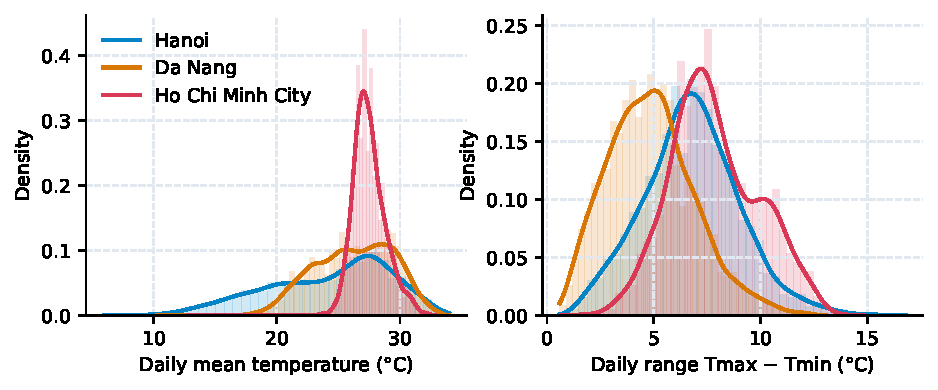
\includegraphics[width=\linewidth]{distributions}
\caption{Histograms (bars) with kernel density estimates (lines) of the daily mean temperature and the DTR.}
\label{fig:dist}
\end{figure}

\subsection{Seasonal cycle}
\begin{figure}[H]
\centering
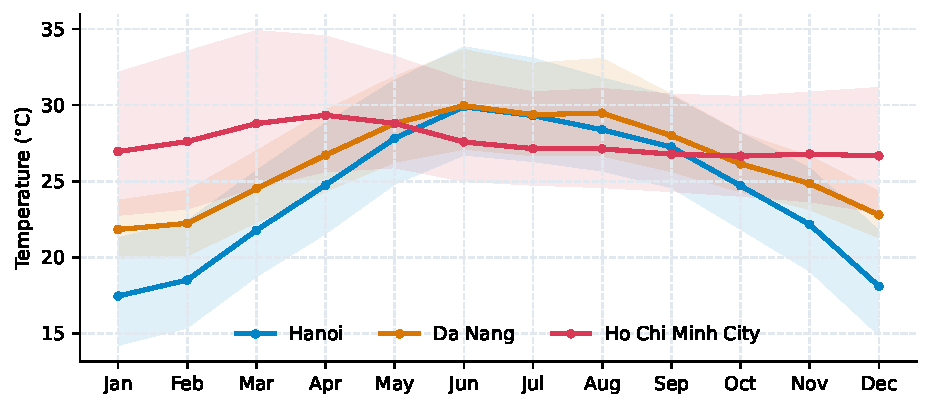
\includegraphics[width=\linewidth]{seasonal_cycle}
\caption{10-year monthly mean temperature (line) and the average daily minimum--maximum (band).}
\label{fig:seasonal}
\end{figure}

Figure~\ref{fig:seasonal} answers the first ``why'' question:
\begin{itemize}
    \item \HN{} goes from 17.5\,\textdegree C in January to 29.9\,\textdegree C in June. It had 585 days with $T_{\min}<15$\,\textdegree C,
    while HCMC had none. The coldest day was 2016-01-24 with $T_{\min}=4.7$\,\textdegree C.
    \item \DN{} follows the same shape as Hanoi but with a smaller amplitude (8.1\,\textdegree C). The sea keeps its winter milder.
    \item \HCM{} is nearly flat (amplitude 2.7\,\textdegree C). It is warmest in April, \emph{before} the rainy season,
    and slightly cooler during the wet months June--December.
    \item From June to August all three cities are about equally warm (27--30\,\textdegree C).
    The difference between the cities is therefore mainly a \emph{winter} difference.
\end{itemize}
Daylight duration follows the sun's position. It is strongly correlated with the daily mean temperature in Hanoi ($r=0.79$) and Da Nang ($r=0.83$),
but only weakly in HCMC ($r=0.30$). Close to the equator, day length changes too little over the year to drive the temperature.
The northern winter is also very cloudy: Hanoi receives only 4.3--4.5 hours of sunshine per day from January to March (Figure~\ref{fig:humsun}).
This reduced sunshine strengthens the cold surges.

The anomaly heatmap (Figure~\ref{fig:anom}) shows that most of the year-to-year variability comes from Hanoi's winter months.
Examples are the very warm February 2019 (+3.5\,\textdegree C) and April 2024 (+3.2\,\textdegree C), and the cold February 2022 ($-3.5$\,\textdegree C) and February 2016 ($-2.9$\,\textdegree C). HCMC's anomalies stay small.

\begin{figure}[H]
\centering
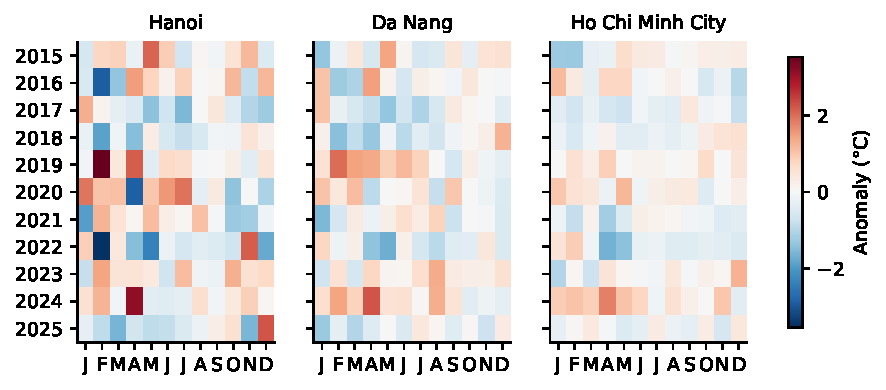
\includegraphics[width=\linewidth]{anomaly_heatmap}
\caption{Monthly temperature anomaly relative to the 10-year mean of the same month (diverging colour map centred on 0).}
\label{fig:anom}
\end{figure}

\subsection{Diurnal temperature range (Tmax $-$ Tmin)}
\begin{figure}[H]
\centering
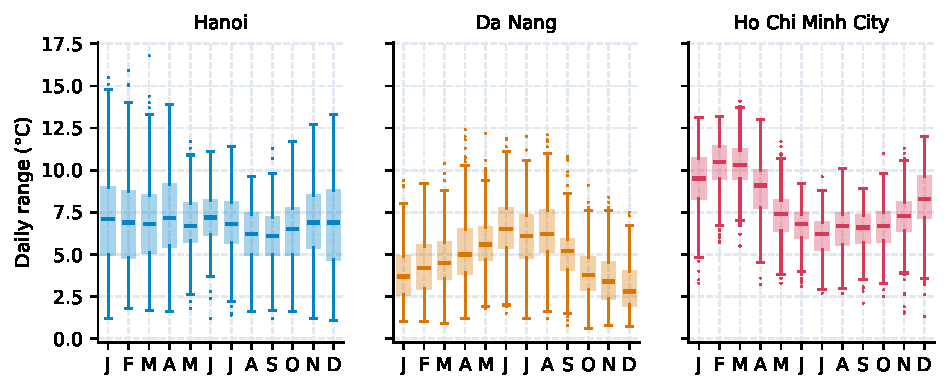
\includegraphics[width=\linewidth]{dtr_boxplots}
\caption{Monthly box plots of the DTR as small multiples with a shared y-axis. Outliers are drawn as points.}
\label{fig:dtr}
\end{figure}

Figure~\ref{fig:dtr} answers the second ``why'' question:
\begin{itemize}
    \item \HCM{} has the largest DTR, but only in its \textbf{dry season}. The median is 9.5--10.5\,\textdegree C from January to March,
    against 6.2--6.8\,\textdegree C from June to September (dry season mean 9.1 vs.\ wet season 6.6\,\textdegree C).
    \item \DN{} has the smallest DTR all year, with a minimum of 2.8\,\textdegree C in December, during its rainy season.
    \item \HN{} has an almost constant median of 6--7\,\textdegree C. Its \emph{spread} in winter, however, is twice as large as in summer
    (IQR 4.0 vs.\ 2.0\,\textdegree C). Winter days can be very cloudy, which gives a small range, or clear and dry after a cold front, which gives a large range.
\end{itemize}

\paragraph{Correction of the proposal's hypothesis.}
The proposal expected HCMC to have a \emph{small} DTR because humidity keeps heat in overnight. The proposed \emph{mechanism}
is supported by the data, but the expected \emph{outcome} is not. HCMC is not humid all year. In its dry season the relative humidity
drops to 64--69\,\% (Figure~\ref{fig:humsun}), and on such dry, sunny days the DTR is large.

\subsection{Drivers of the daily range}
\begin{figure}[H]
\centering
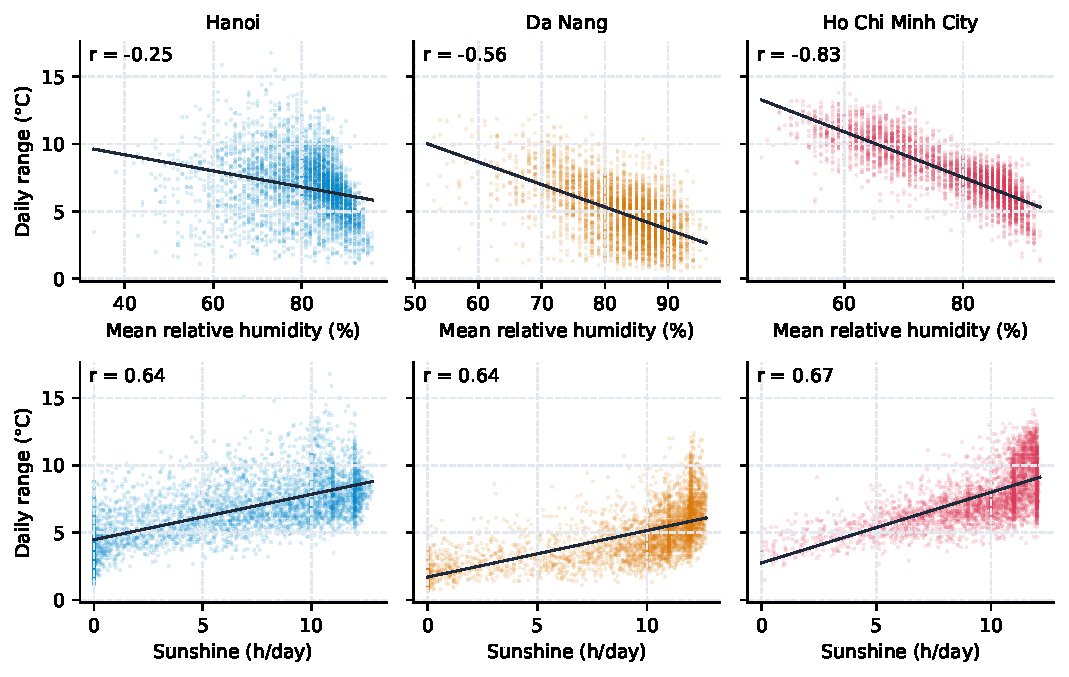
\includegraphics[width=\linewidth]{drivers_scatter}
\caption{DTR against mean relative humidity (top) and sunshine duration (bottom), one panel per city, with least-squares lines.}
\label{fig:drivers}
\end{figure}

\begin{figure}[H]
\centering
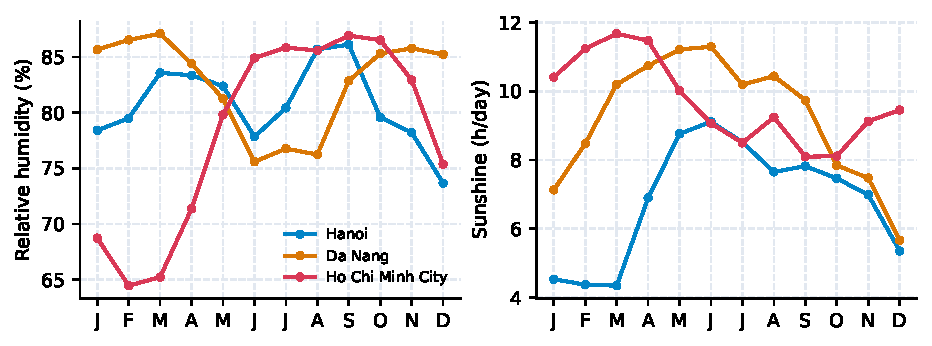
\includegraphics[width=\linewidth]{humidity_sunshine}
\caption{Monthly mean relative humidity and sunshine duration.}
\label{fig:humsun}
\end{figure}

\begin{table}[H]
\centering\small
\begin{tabular}{lrrr}
\toprule
Pearson $r$ with DTR & Humidity & Sunshine & Precipitation \\
\midrule
\HN  & $-0.25$ & $0.64$ & $-0.34$ \\
\DN  & $-0.56$ & $0.64$ & $-0.38$ \\
\HCM & $-0.83$ & $0.67$ & $-0.54$ \\
\bottomrule
\end{tabular}
\caption{Correlation of daily drivers with the DTR (Spearman $\rho$ gives the same picture, see \texttt{stats.txt}).}
\label{tab:corr}
\end{table}

Sunshine is a consistent positive driver in all three cities ($r\approx0.65$): a sunny day heats up strongly during the day.
Humidity has a strong effect in HCMC ($r=-0.83$) but only a weak one in Hanoi ($r=-0.25$).
In Hanoi, cloud cover and cold-air advection play a larger role than humidity.
These are correlations, not causal effects. Humidity, cloud and rain all change together with the monsoon season.

\subsection{Day-to-day changes}
\begin{figure}[H]
\centering
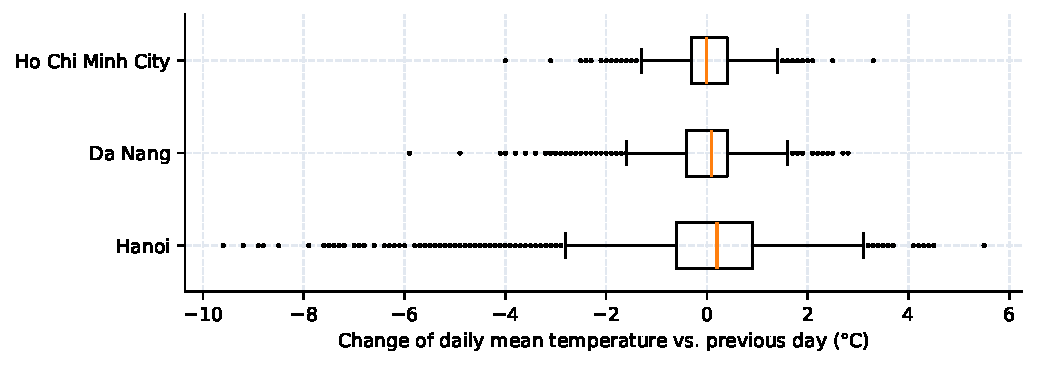
\includegraphics[width=\linewidth]{day_to_day}
\caption{Distribution of the day-to-day change of the daily mean temperature.}
\label{fig:dT}
\end{figure}

Hanoi's mean temperature changes by 1.11\,\textdegree C per day on average. Da Nang changes by 0.53\,\textdegree C and HCMC by 0.44\,\textdegree C.
Large drops of at least 4\,\textdegree C within one day happened 117 times in Hanoi, 4 times in Da Nang and once in HCMC.
The largest drop was $-9.6$\,\textdegree C in Hanoi.
These drops are cold surges of the winter north-east monsoon, so the weather in Hanoi is much less predictable from one day to the next.

\subsection{Interannual trends}
\begin{figure}[H]
\centering
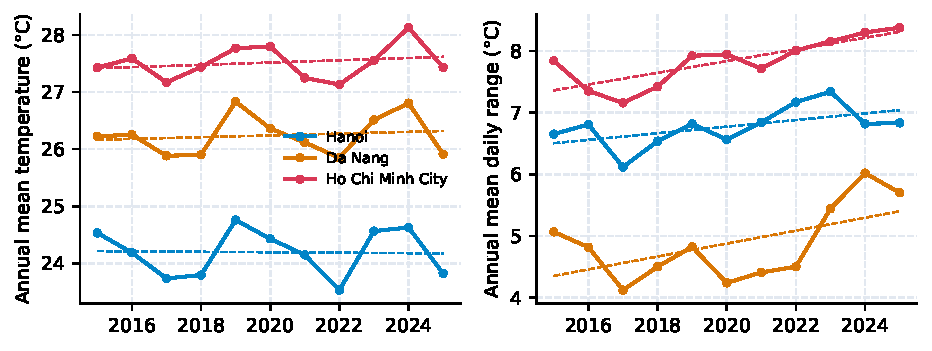
\includegraphics[width=\linewidth]{annual_trends}
\caption{Annual mean temperature and annual mean DTR with linear trends (dashed).}
\label{fig:trend}
\end{figure}

None of the cities shows a significant trend in the annual mean temperature (all $p>0.5$).
The DTR, however, \emph{increases} in all three cities: by +0.54, +1.05 and +0.95\,\textdegree C per decade.
For HCMC this increase is significant (OLS $p=0.003$, Mann--Kendall $\tau=0.75$, $p=0.001$).
It comes from a rising $T_{\max}$ (+0.83\,\textdegree C/decade) together with a flat $T_{\min}$.
11 years is a short period and the data is reanalysis, so this trend should be treated as a hint and not as a climate signal.
It connects to RQ3 (hot days), because a higher $T_{\max}$ directly increases the number of days above 35\,\textdegree C.
Global warming is about 0.2\,\textdegree C per decade, which is smaller than the year-to-year swings caused by El Niño (next section).
Detecting it would need at least 30 years of data; the Open-Meteo archive goes back to 1940.

\subsection{El Niño and La Niña}
The warm years 2019 and 2024 and the cold year 2022 suggest a link to the El Niño--Southern Oscillation (ENSO).
We added NOAA's \textbf{Oceanic Niño Index} (ONI; \texttt{data/oni.csv}), the 3-month mean sea-surface temperature anomaly
in the central tropical Pacific. Months with ONI $\ge+0.5$\,\textdegree C count as El Niño and months with ONI $\le-0.5$\,\textdegree C as La Niña.
The period contains three El Niño events (2014--16, very strong; 2018--20, moderate; 2023--24, strong) and two La Niña events (2017--18; 2020--23).
We compared the ONI with the monthly temperature anomaly of each city (the month's mean minus the 10-year mean of that month).

\begin{figure}[H]
\centering
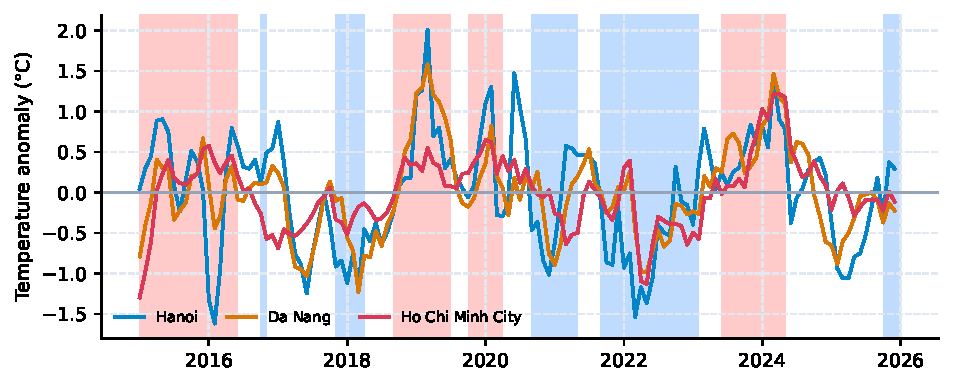
\includegraphics[width=\linewidth]{elnino}
\caption{Monthly temperature anomaly (3-month centred mean) with El Niño (red) and La Niña (blue) months shaded.}
\label{fig:elnino}
\end{figure}

\begin{table}[H]
\centering\small
\begin{tabular}{lrrrrrr}
\toprule
 & \multicolumn{3}{c}{\shortstack{$r$ with ONI\\lead $n$ months}} & \multicolumn{3}{c}{Mean anomaly (lag 3 months)} \\
\cmidrule(lr){2-4}\cmidrule(lr){5-7}
City & $n=0$ & $n=2$ & $n=4$ & La Niña & Neutral & El Niño \\
\midrule
\HN  & 0.20 & 0.21 & 0.21 & $-0.30$ & $-0.18$ & $+0.40$ \\
\DN  & 0.32 & 0.37 & 0.37 & $-0.34$ & $-0.12$ & $+0.37$ \\
\HCM & 0.42 & 0.50 & 0.53 & $-0.32$ & $-0.08$ & $+0.30$ \\
\bottomrule
\end{tabular}
\caption{Link between ENSO and monthly temperature anomalies (\textdegree C). 47 El Niño, 54 neutral and 31 La Niña months.}
\label{tab:enso}
\end{table}

\begin{itemize}
    \item \textbf{El Niño warms, La Niña cools all three cities} by a similar amount: the difference between the two phases is 0.6--0.7\,\textdegree C.
    \item \textbf{The effect is delayed.} The correlation is highest when the ONI leads by 2--4 months (HCMC $r=0.53$), because the ocean
    heat needs time to change the circulation over South-East Asia.
    \item \textbf{HCMC follows ENSO most closely, Hanoi least.} In HCMC, El Niño also brings about 25\,mm less rain per month and lower
    humidity. In Hanoi ($r=0.2$), the winter cold surges (Section~3.5) override the ENSO signal; for example, the very strong El Niño of 2015--16
    did not prevent the record cold of January 2016.
    \item \textbf{The effect is strongest in spring} (Mar--May, averaged over the cities): $+0.53$\,\textdegree C in El Niño vs.\ $-0.38$\,\textdegree C in La Niña months.
    \item \textbf{Consequence for the trend question:} the warm peak of 2023--24 and the hotter extremes in Da Nang and HCMC in recent years
    are largely El Niño effects. Within 11 years, ENSO cannot be separated from long-term warming.
\end{itemize}
With only five events, these numbers describe tendencies rather than precise effects.

%=====================================================================
\section{Visualization Design Options}
We compared several encodings for RQ1 using the principles from the course:
expressiveness and effectiveness, Cleveland \& McGill's ranking of channels (position on a common aligned scale first),
Tufte's data-ink ratio and graphical integrity, small multiples (``eyes beat memory''),
linked views, and Shneiderman's mantra (\emph{overview first, zoom and filter, details on demand}).

\begin{table}[H]
\centering\small
\begin{tabularx}{\linewidth}{>{\raggedright}p{3.2cm}>{\raggedright}X>{\raggedright\arraybackslash}X c}
\toprule
Option & Strength & Weakness & Used \\
\midrule
Annual line chart with drill-down (existing) & Overview + zoom to month and day; shows day-to-day changes & Annual means hide the seasons, which carry the main differences & \checkmark \\
Seasonal multi-line + min/max band & Mean on a common scale; band width shows the DTR & Bands of three cities overlap and become muddy & replaced \\
Monthly min--max bars per city (``fingerprint'') & Level, seasonality and DTR in one encoding, no overlap & 36 bars; the reader needs the legend line to decode it & \checkmark \\
Year $\times$ month anomaly heatmap & Shows all 132 months; unusual months stand out & Colour is less precise than position; needs a diverging map & \checkmark \\
Anomaly timeline with ENSO shading, drop ticks and brush & El Niño, its delay and day-to-day volatility on one time axis; zoomable & Monthly anomalies are noisy (3-month smoothing needed) & \checkmark \\
Monthly box plots (small multiples) & Median, IQR and outliers per month; shared y-axis & Hides multimodality (course: ``one box plot, four distributions'') & \checkmark \\
Violin / KDE plots & Show the shape of the distribution & 36 violins are hard to read; results depend on the bandwidth & report \\
Histogram per city & Simple, honest & The number of bins changes the picture; no seasonal dimension & report \\
Dual-axis chart (sunshine vs.\ temp.) & Compact & Two y-scales suggest false relationships; hard to read & no \\
Scatter DTR vs.\ driver (small multiples) & Shows the relationship and its strength per city & 4\,000 points per panel cause overplotting & \checkmark \\
\bottomrule
\end{tabularx}
\caption{Candidate visualizations for RQ1.}
\end{table}

We replaced the proposal's dual-axis sunshine chart with a \emph{driver selector} (humidity or sunshine) on the scatter plots.
This keeps one variable per axis and avoids comparing two scales against each other.

%=====================================================================
\section{Implemented Dashboard}
The \emph{Temperature Dynamics \& Variations} tab follows Shneiderman's mantra: two overview charts with the key insights first,
then detail views for zooming, filtering and details on demand. One set of city checkboxes at the top filters every chart.

\subsection*{Key Insights}
Two charts summarise the findings (Figure~\ref{fig:insights}):
\begin{enumerate}
    \item \textbf{A typical year (``fingerprint'')}: for each month and city, a bar from the average daily minimum to the average
    daily maximum, with a tick and a thin line for the monthly mean. One encoding shows three findings: the \emph{position} of the bars
    gives the level, their \emph{movement} over the year the seasonality, and their \emph{length} the daily range.
    The tooltip adds that month's humidity and sunshine, so the explanation is one hover away.
    This chart replaces an earlier seasonal line chart whose min--max bands overlapped.
    \item \textbf{2015--2025}: the 3-month smoothed monthly anomaly per city, with El Niño and La Niña periods shaded.
    Below it, one lane per city has a tick for every day on which the mean fell by 4\,\textdegree C or more.
    A small strip at the bottom shows the whole period; dragging in it zooms the chart above (overview + detail).
\end{enumerate}
\subsection*{Explore the Details}
\begin{enumerate}
    \item \textbf{Annual, monthly and daily mean temperature} (the original chart): drill-down from years to months to days,
    with breadcrumb navigation.
    \item \textbf{Unusually warm or cold months}: a year $\times$ month heatmap per city of the anomaly from the 10-year monthly average,
    on a shared diverging scale centred on 0. Clicking a cell opens that month's daily temperatures in the drill-down chart.
    \item \textbf{Daily range by month}: box plots as small multiples, one panel per city on a shared y-axis, with outliers drawn as circles.
    \item \textbf{Drivers}: scatter plots of DTR against humidity or sunshine, one panel per city, each with a regression line and Pearson $r$.
\end{enumerate}
Hovering a month in the heatmap or a box plot highlights the same month in all three detail views (linked highlighting).
For example, hovering February shows that HCMC's large dry-season DTR comes from its sunniest days (Figure~\ref{fig:linked}).

\paragraph{Design decisions.}
\begin{itemize}
    \item \textbf{Position first:} all quantitative values except the heatmap anomalies are encoded by position on aligned, shared scales.
    Colour encodes the city, and in the heatmap the anomaly (with exact values in the tooltip).
    \item \textbf{Consistent colour:} the team palette (\HN{} blue, \DN{} amber, \HCM{} red) is used on all tabs. City names are always written
    as text too, so the charts can be read without telling the colours apart (amber and red can be confused under deuteranopia).
    \item \textbf{Data-ink:} light dashed gridlines, no chart borders, no 3D or decoration.
    \item \textbf{Integrity:} the y-axis of the box plots and the scatter plots starts at 0 because the DTR is a magnitude.
    Temperature charts use a fitted range, which is common practice for interval data.
    \item \textbf{Overplotting:} small, semi-transparent points (opacity 0.25) are used for the 12\,054 daily observations.
\end{itemize}

\paragraph{Code.}
The temperature charts are in \texttt{js/temperature.js} (shared helpers and detail charts) and \texttt{js/temperatureInsights.js}
(Key Insights). The only changes to shared files are:
(i) three new fields (\texttt{tempMin}, \texttt{humidity}, \texttt{sunshineHours}) on the parsed rows in \texttt{dataLoader.js},
(ii) in \texttt{main.js}, two event registrations plus changes inside the existing temperature function \texttt{drawTemperatureChart}
(breadcrumb navigation and opening a month selected in the heatmap),
(iii) new markup inside the temperature section of \texttt{index.html},
(iv) new CSS classes prefixed with \texttt{temperature-}, and
(v) the new file \texttt{data/oni.csv} with the NOAA El Niño index for 2014--2025.
The rainfall and extreme-weather code was not changed.

\begin{figure}[H]
\centering
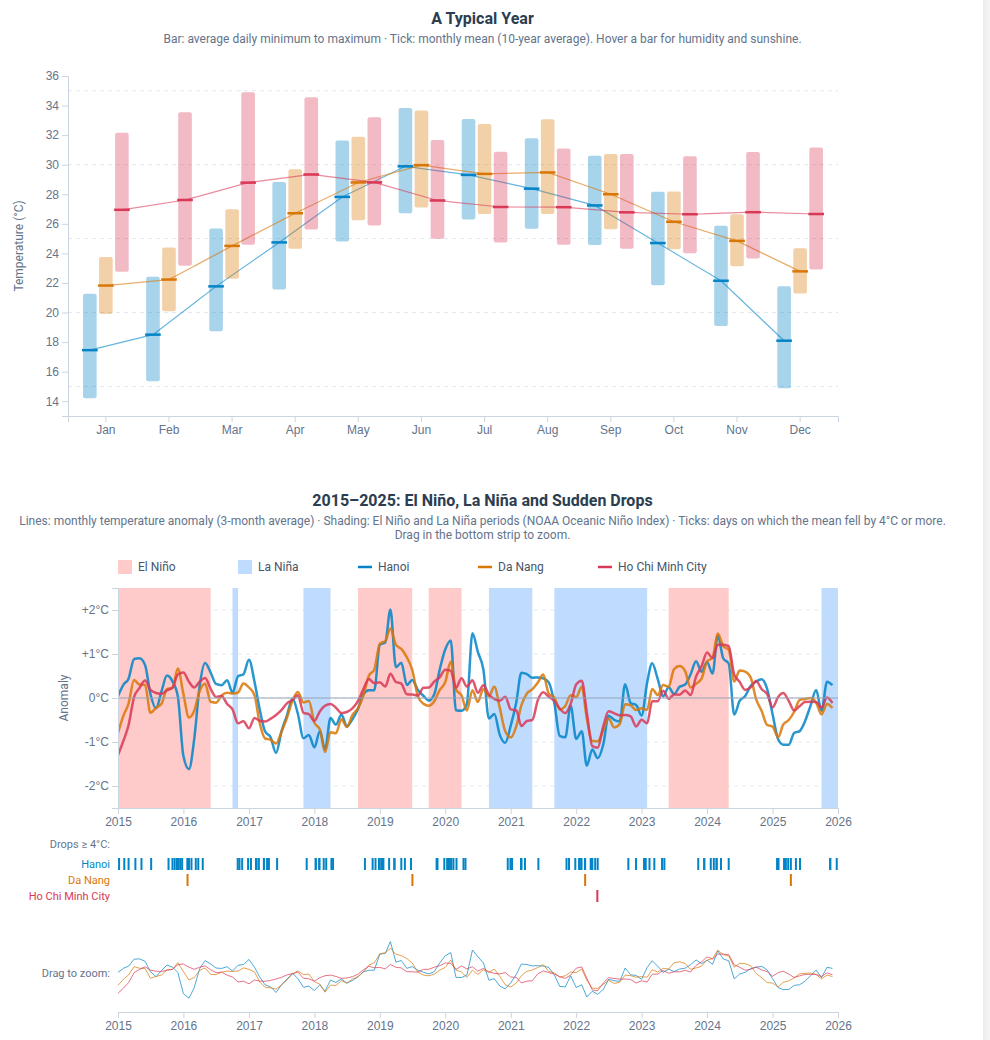
\includegraphics[width=0.9\linewidth,height=0.75\textheight,keepaspectratio]{dashboard_insights}
\caption{The two Key Insights charts: a typical year, and 2015--2025 with El Niño periods and sudden drops.}
\label{fig:insights}
\end{figure}

\begin{figure}[H]
\centering
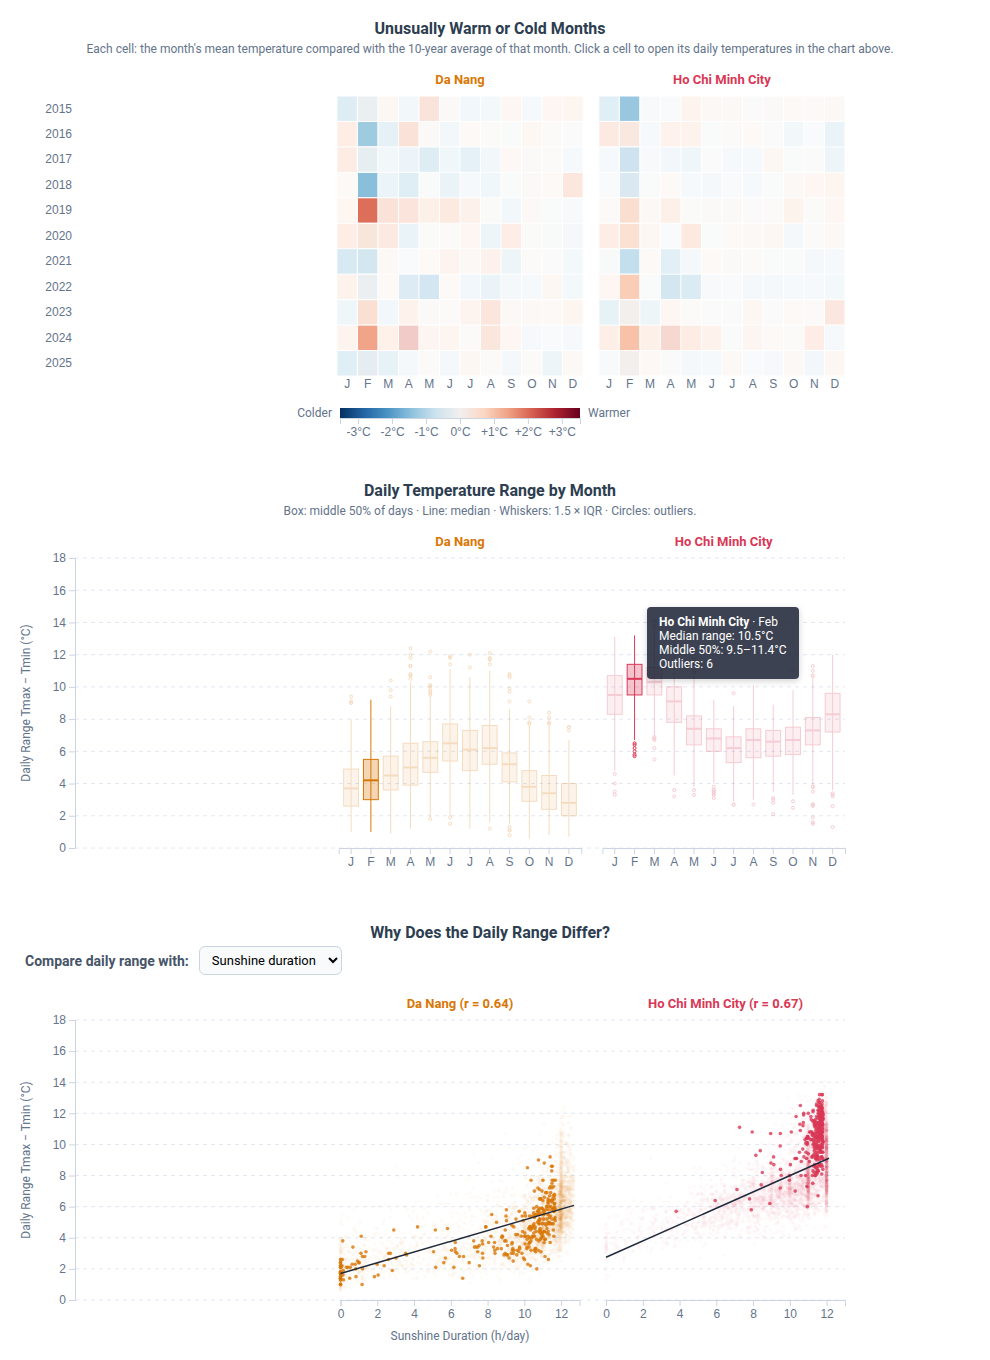
\includegraphics[width=0.9\linewidth,height=0.75\textheight,keepaspectratio]{dashboard_linked}
\caption{Linked detail views: Hanoi filtered out, sunshine selected as the driver, and February hovered in the HCMC box plot.
The same month is highlighted in the heatmap and the scatter plots.}
\label{fig:linked}
\end{figure}

%=====================================================================
\section{Conclusion}
\begin{itemize}
    \item \textbf{Level:} HCMC (27.5\,\textdegree C) $>$ Da Nang (26.2) $>$ Hanoi (24.2). The gap comes almost entirely from winter.
    In summer the three cities are about equally warm.
    \item \textbf{Seasonality:} Hanoi has a 12.4\,\textdegree C seasonal swing and frequent cold surges, Da Nang a moderated one (8.1),
    and HCMC almost none (2.7). The main driver is latitude: day length and sun angle.
    \item \textbf{Daily range:} HCMC has the largest DTR (7.8\,\textdegree C) because of its dry, sunny season.
    Coastal Da Nang has the smallest (4.9\,\textdegree C). Humidity and sunshine together explain much of the DTR, especially in HCMC.
    \item \textbf{Day-to-day changes:} Hanoi changes about twice as much from one day to the next as the other two cities.
    \item \textbf{Trend:} no measurable warming of the mean over 11 years, but a widening DTR (significant in HCMC) driven by a rising $T_{\max}$.
    \item \textbf{El Niño:} El Niño months are about 0.6--0.7\,\textdegree C warmer than La Niña months, with a delay of 2--4 months.
    The link is strongest in HCMC and weakest in Hanoi, and it explains most of the year-to-year ups and downs, such as the warm years 2019 and 2024.
\end{itemize}

\paragraph{Limitations.}
The data is gridded reanalysis and not station data. The values represent grid cells and can underestimate local extremes.
11 years is too short for robust climate trends, and the period contains only five ENSO events.
The correlations describe co-occurrence with the seasons, not causality.

\end{document}
